% !TeX program = LuaLaTeX
\documentclass[parskip=half]{scrartcl}

\input{../name}

\usepackage{xcolor}
\usepackage{hyperref}
\hypersetup{
    colorlinks,
    linkcolor={red!50!black},
    citecolor={blue!50!black},
    urlcolor={blue!80!black}
}

\usepackage{graphicx}
\graphicspath{ {./images/} }

\usepackage{datetime2}

% Font Stuff

\usepackage{microtype}
\usepackage{fontspec}
\usepackage{unicode-math}

% Stix fonts should be auto-installed by the TeX package manager
\setmainfont{Georgia}
\setmonofont{Source Code Pro}
\setmathfont{Stix Two Math} 

% Stylistically a good match, and licensed under the Open Font License
\setsansfont{Helvetica Neue}

\newcommand{\figref}[1]{Figure~\ref{#1}}

\begin{document}

{\LARGE \textbf{\textsf{Vulnerability Report (HW2)}}}
\vspace*{1em}

\textbf{Date:} 2023-05-25

\textbf{Author:} \docauthor

\textbf{Student code:} \texttt{\studentcode}

Notes:
\begin{enumerate}
    \item The actual student code is not present in the web application
    database. I have assumed the student code \texttt{C18947} for this task.
    \item I do not reproach HTTP availability in this report, since this is
    (I assume) for operational convenience.
\end{enumerate}

This report has $8$ pages.

\section*{Vulnerability 1}\label{vuln1}

\textbf{Risk level.} critical

Access control is performed based on the account holder's name. Account holder
names themselves are not restricted/validated.

\textbf{Risk.} An attacker is able to access some protected website areas
without proper authorisation, and therefore see information they are not privy
to. In this case, the attacker can see the list of all signed up users, and
get their names and email addresses, which is a privacy breach.

The attack vector is broken access control, insecure design. Namely, an
attacker simply has to create an account with the name of the administrative
user, and can then access some administrative page without actual
administrative privileges. The attacker can do this by brute-forcing/guessing
some names, however the attack is trivial with access to source code.

The function \texttt{admin()} in the source code file \texttt{main.py} contains
part of the flawed logic. Particularly, line $25$ contains the flawed
permission logic, where access is evaluated based on the account's name.
The function's source code is shown in \figref{fig:code:admincomp}.

\begin{figure}[h]
    \centering
    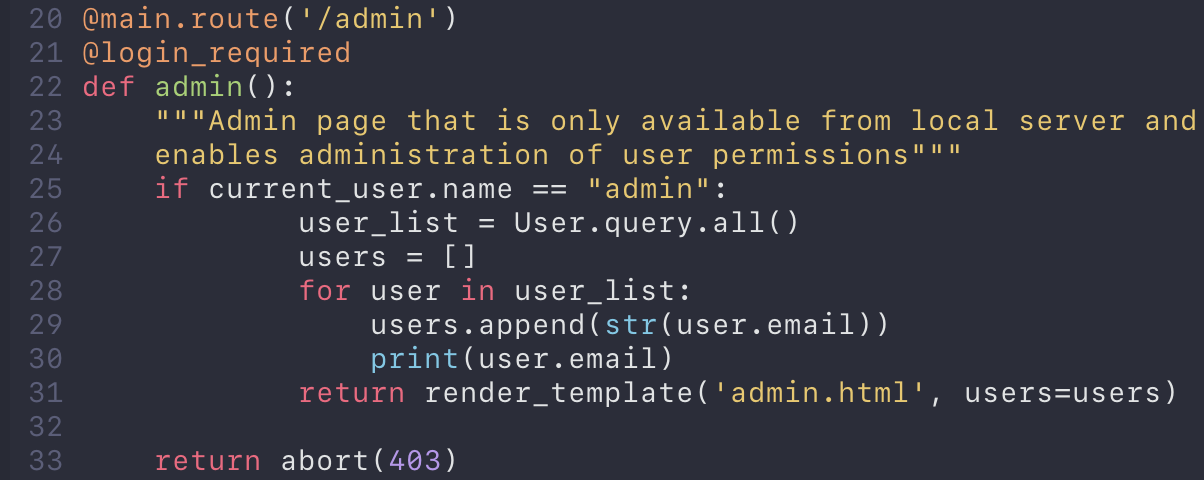
\includegraphics[width=\textwidth]{code_admincomp}
    \caption{Name-based access control}
    \label{fig:code:admincomp}
\end{figure}

Because there is nothing preventing a user from creating an account with name
``admin'', the access control validation can easily be exploited. User account
creation is handled by the function \texttt{signup\_post()} in the file
\texttt{auth.py}, and is shown in \figref{fig:code:signup}.

\begin{figure}[h]
    \centering
    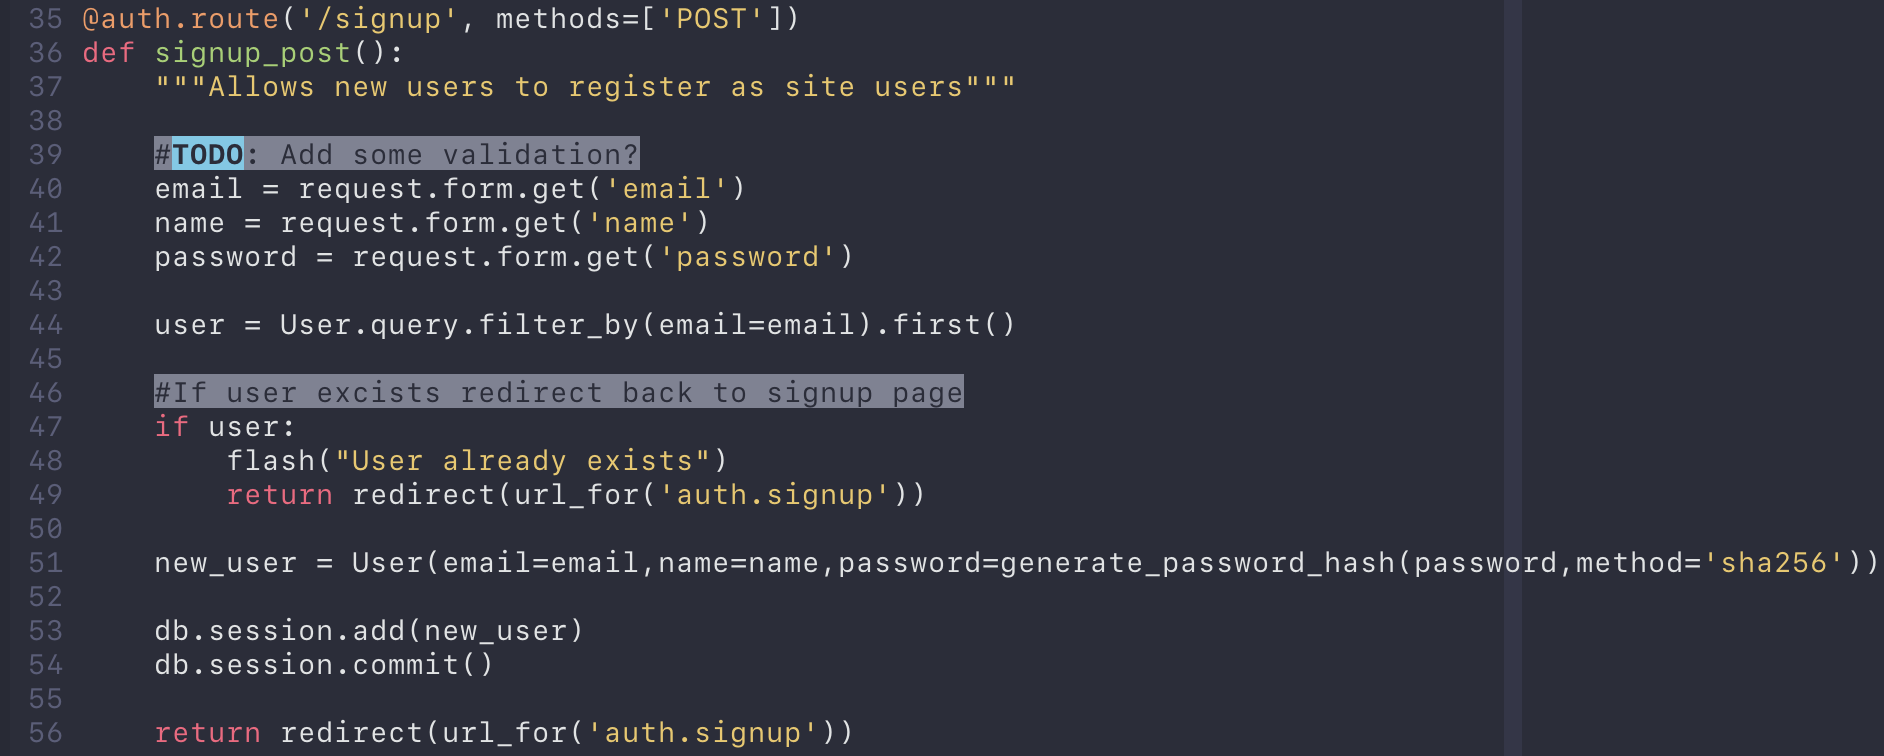
\includegraphics[width=\textwidth]{code_acccreate}
    \caption{Account signup with lacking validation}
    \label{fig:code:signup}
\end{figure}

Potentially applicable OWASP categories are:
\begin{enumerate}
  \item \texttt{A01:2021} -- Broken Access Control%\footnote{\url{https://owasp.org/Top10/A01_2021-Broken_Access_Control/}}
  \item \texttt{A04:2021} -- Insecure Design%\footnote{\url{https://owasp.org/Top10/A04_2021-Insecure_Design/}}
\end{enumerate}

\textbf{Proof of Concept.}

Exploitation is carried out in three steps:
\begin{enumerate}
    \item register a user account with name ``admin'' (\figref{fig:sigadm}),
    \item log-in with this user account,
    \item access \texttt{localhost:8080/admin} and see signed up accounts
    (\figref{fig:viewadm}).
\end{enumerate}

\begin{figure}[h]
    \centering
    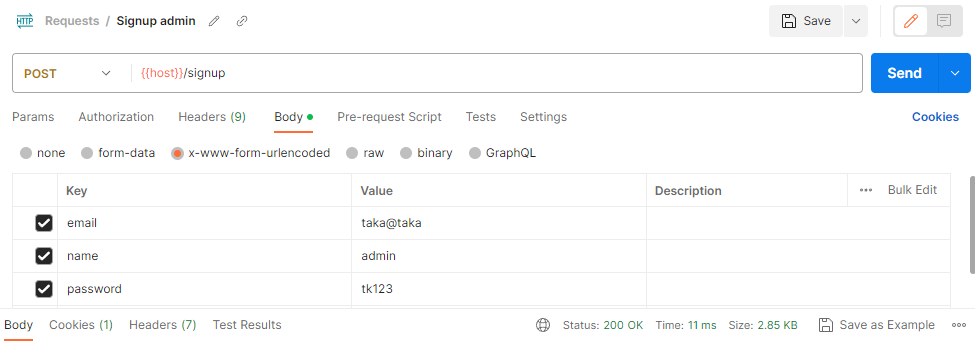
\includegraphics[width=\textwidth]{signup_admin}
    \caption{Sign up with name ``admin''}
    \label{fig:sigadm}
\end{figure}

\begin{figure}[h]
    \centering
    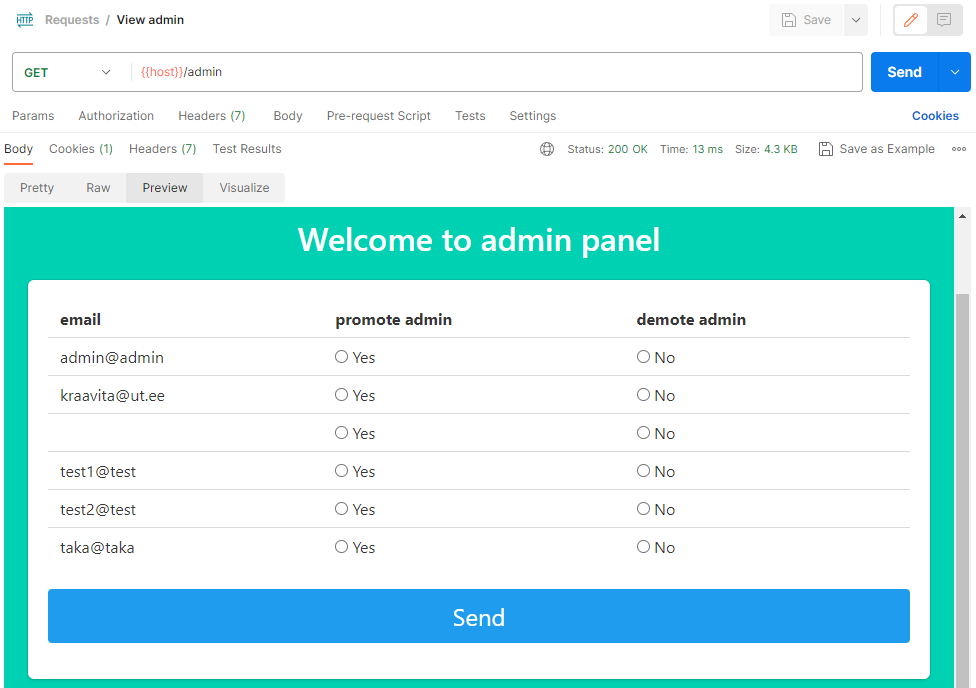
\includegraphics[width=\textwidth]{view_admin}
    \caption{View all user accounts}
    \label{fig:viewadm}
\end{figure}

\textbf{Recommendations.} Implement proper access control, e.g., role-based or
attribute-based. That is, allow access to resources only by validating specific
permission rules, instead of arbitrary attributes. Enforce this proper access
control consistently across the system.

For the given source code, the check on line $25$ should be replaced with
\begin{verbatim}
current_user.isadmin == 1
\end{verbatim}

\clearpage
\newpage

\section*{Vulnerability 2}

\textbf{Risk level.} critical

%No permission validation is performed for a critical administrative operation.
Administrative privileges of user accounts may be set or unset without prior
authentication and authorisation.

\textbf{Risk.} An attacker can promote any regular user account to an
administrative account, and can demote all administrators to regular users.

The attack vector is a lack of authentication and missing access control. The
server allows queries to an administrative endpoint for unauthenticated users,
and blindly executes those queries without any form of permission validation.

Potentially applicable OWASP categories are:
\begin{enumerate}
  \item \texttt{A07:2021} -- Identification and Authentication Failures%\footnote{\url{https://owasp.org/Top10/A07_2021-Identification_and_Authentication_Failures/}}
  \item \texttt{A01:2021} -- Broken Access Control%\footnote{\url{https://owasp.org/Top10/A01_2021-Broken_Access_Control/}}
  \item \texttt{A04:2021} -- Insecure Design%\footnote{\url{https://owasp.org/Top10/A04_2021-Insecure_Design/}}
\end{enumerate}

\textbf{Proof of Concept.}

The function \texttt{admin\_get()} in the source code file \texttt{main.py}
contains the logic for managing the administrative privileges of user accounts.
The function's source code is shown in \figref{fig:code:adminset}.

\begin{figure}[h]
    \centering
    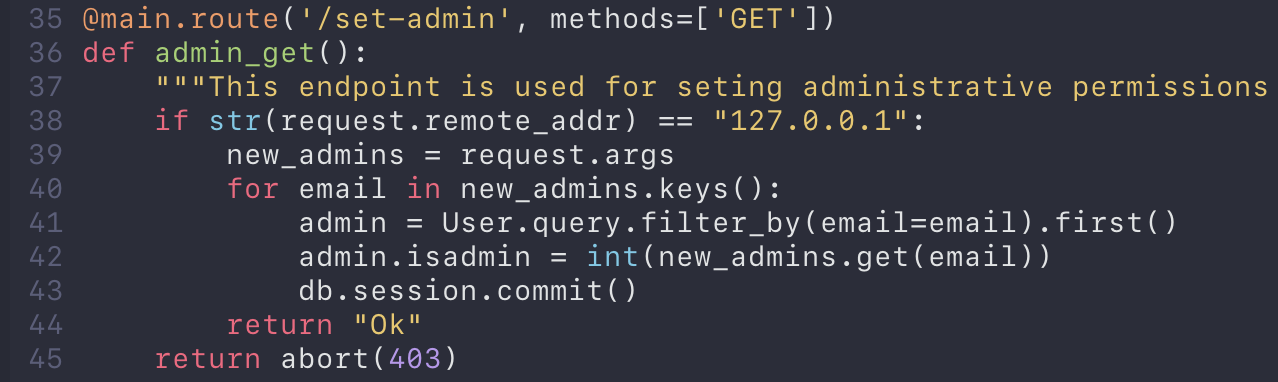
\includegraphics[width=\textwidth]{code_adminset}
    \caption{Privilege management without authentication and authorisation}
    \label{fig:code:adminset}
\end{figure}

To exploit the vulnerability, one may simply make a \texttt{GET} request to
\begin{verbatim}
localhost:8080/set-admin?<email>=<flag>
\end{verbatim}
where \texttt{<email>} is the email address of the desired user account to
change permissions for, and \texttt{<flag>} is $1$ to enable privileges or $0$
to remove privileges.

For example, consider the regular user with email \texttt{\email}. This user
can view user grades (\figref{fig:grades:view}) but cannot change these
grades (\figref{fig:grades:failupdate}).

\begin{figure}[h]
    \centering
    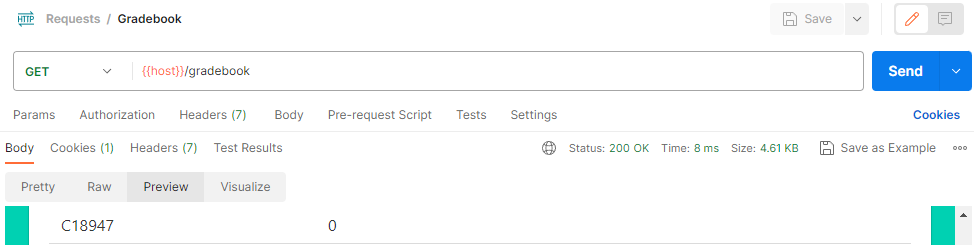
\includegraphics[width=\textwidth]{view_grade}
    \caption{Initial grades view}
    \label{fig:grades:view}
\end{figure}

\begin{figure}[h]
    \centering
    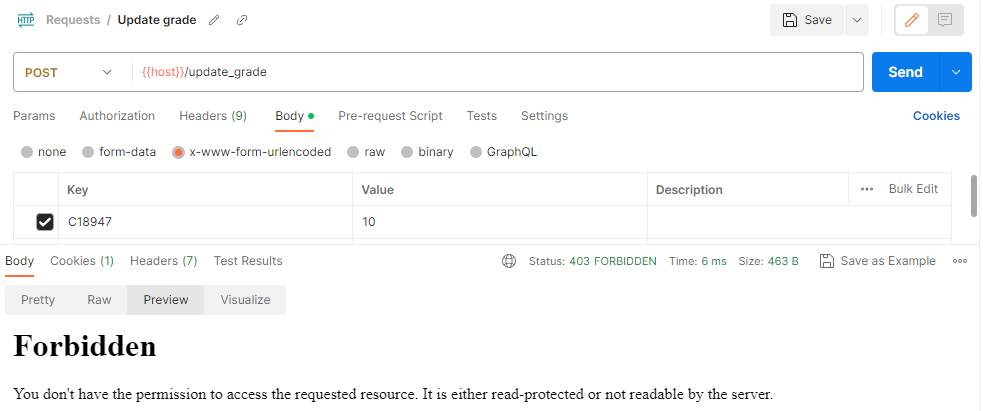
\includegraphics[width=\textwidth]{forbidden_grade}
    \caption{Unauthorised grade modification}
    \label{fig:grades:failupdate}
\end{figure}

However, with a \texttt{GET} request to the \texttt{/set-admin} endpoint
(\figref{fig:setadmin}) the user is given administrative privileges, and the
user can subsequently update grades (\figref{fig:grades:update}).

\begin{figure}[h]
    \centering
    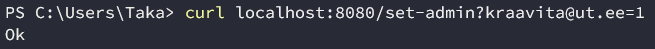
\includegraphics[width=\textwidth]{set_admin}
    \caption{Permission elevation}
    \label{fig:setadmin}
\end{figure}

\begin{figure}[h]
    \centering
    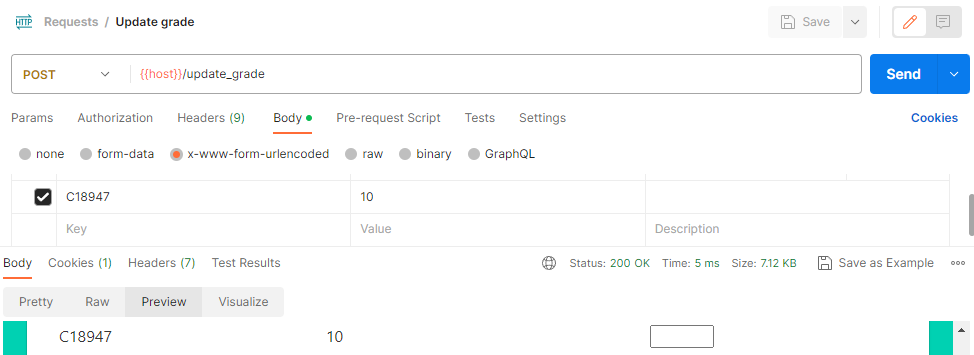
\includegraphics[width=\textwidth]{view_new_grade}
    \caption{Authorised grade modification}
    \label{fig:grades:update}
\end{figure}

\textbf{Recommendations.} Do not allow requests to endpoints designed for
access or modification of some internal data/state without prior
authentication. This must hold true for both administrative actions but also
regular user actions. Moreover, validate permissions for all requests, i.e.,
always verify whether an entity is allowed to access and/or operate on some
data.

For the given source code, the function should be preceded by
\begin{verbatim}
@login_required
\end{verbatim}
and the check on line $38$ should be replaced with
\begin{verbatim}
current_user.isadmin == 1
\end{verbatim}

% Do not allow GET requests to change the system state.

\clearpage
\newpage

\section*{Vulnerability 3}

\textbf{Risk level.} high

Data is validated only on the client side. There is no server-side validation.

\textbf{Risk.} The server can be made to store data that makes no sense
business-logic wise, and may lead to erroneous data processing. Suppose that
the average course grade of students is calculated as the arithmetic average of
the grades of all students. But, if one student is made to have a grade of
more than a million points, this result is completely skewed.

The attack vector is the lack of server-side input validation. This leaves the
server open to injection attacks, and invalid states for business logic.

\textbf{Proof of Concept.}

One can sign up with an empty email (one such user is shown in
\figref{fig:viewadm}), or can make a student have the grade $987654321$ by
submitting data to the server endpoint directly. \figref{fig:grades:absurd}
shows the submission of ridiculous data, while \figref{fig:grades:bound} shows
that values are validated on the client-side.

\begin{figure}[h]
    \centering
    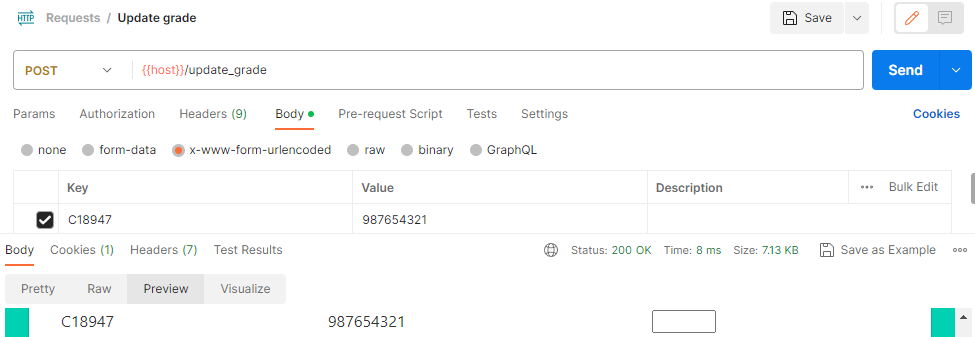
\includegraphics[width=\textwidth]{absurd_grade}
    \caption{Lack of server side grade validation}
    \label{fig:grades:absurd}
\end{figure}

\begin{figure}[h]
    \centering
    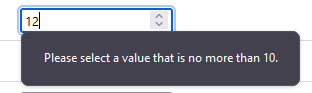
\includegraphics[width=200pt]{value_bound}
    \caption{Client side grade validation}
    \label{fig:grades:bound}
\end{figure}

\textbf{Recommendations.} Perform at least the same data validations server
side which are done on the client side. More generally, validate all user
created data for business logic and security on the server side. This also
helps prevent injection attacks.

\end{document}
